\documentclass{sig-alternate}
\usepackage[latin1]{inputenc}
\usepackage{url}
\usepackage{listings}

\begin{document}
%
% --- Author Metadata here ---
\conferenceinfo{GECCO'14} {Vancouver, Canada}
\CopyrightYear{2014}
%\CopyrightYear{2007} % Allows default copyright year (20XX) to be over-ridden - IF NEED BE.
%\crdata{0-12345-67-8/90/01}  % Allows default copyright data (0-89791-88-6/97/05) to be over-ridden - IF NEED BE.
% --- End of Author Metadata ---

\title{Assessing different architectures for evolutionary algorithms in JavaScript}
\subtitle{}

\author{
% \alignauthor
% J.J. Merelo, Pedro Castillo, Antonio Mora\\
%        \affaddr{University of Granada}\\
%        \affaddr{GeNeura, Department of Computer Architecture and Technology, ETSIIT + CITIC}\\
%        \affaddr{18071 - Granada}\\
%        \email{jmerelo,pedro,amorag@geneura.ugr.es}
% \alignauthor
% Anna I. Esparcia-Alc�zar\\
% \affaddr{S2 Grupo}\\
% \email{aesparcia@s2grupo.es}
% \alignauthor
% V�ctor Rivas-Santos\\
% \affaddr{Universidad de Ja�n}\\
% \email{vrivas@ujaen.es}
\alignauthor
Three wise guys\\
       \affaddr{University of Miskatonic}\\
       \affaddr{Wise affairs dep}\\
       \affaddr{Metropolis}\\
       \email{some.good.e@mails.com}
\alignauthor
Another author\\
\affaddr{Adrress}\\
\email{e@ma.il}
\alignauthor
Last one\\
\affaddr{Science Institute}\\
\email{last@o.ne}
}

\maketitle
\begin{abstract}After more than fifteen years, JavaScript has finally risen as a popular
language for implementing all kind of applications, from server-based
to rich Internet Applications. The fact that it is implemented in the browser and in server-side tools makes it interesting for
% Antonio - qu� features en concreto?, al menos n�mbralas
designing evolutionary algorithm frameworks 
that encompass both
tiers, but besides, they allow a change in paradigm that goes beyond
the canonical evolutionary algorithm. 
%Maribel, muchos frameworks van más allá del algoritmo genético canónico, pero esto no pasa porque estén hechos en javascript
% Antonio - qu� cambio en concreto?
In this paper we will experiment
with different architectures, client-server and peer to peer to assess which ones offer most advantages in terms of
performance, scalability and ease of use 
for the computer scientist. All implementations  have been released as open source, and besides showing that the concept of working with evolutionary algorithms in JavaScript can be done efficiently, we prove that a master-slave parallel architecture offers the best combination of time and algorithmic improvements in a parallel evolutionary algorithm that leverages JavaScript implementation features.

\end{abstract}

% A category with the (minimum) three required fields
\category{H.4}{Information Systems Applications}{Miscellaneous}
%A category including the fourth, optional field follows...
\category{D.2.8}{Software Engineering}{Metrics}[complexity measures, performance measures]

\keywords{Javascript, node.js, parallel evolutionary algorithms, asynchronous evolution}

\section{Introduction}

JavaScript (JS from now on) was introduced in 1998 as a browser-oriented language by
Netscape \cite{flanagan1998javascript}; it was quickly adopted, in
several versions, by the rest of the existing browsers (Internet
Explorer, Opera and the offspring of Netscape, Mozilla and then
Firefox). It became a standard by the European Association for
Standardizing Information and Communication Systems in 1999
\cite{ecma1999262}. However, it was for a long time considered just a
language for the browser, and in fact most books on JS
\cite{goodman2007javascript} start by
telling you how to embed your scripts in the browser HTML code.

As such as a embedded language, Javascript is an interpreted language
that uses classes and objects, uses functions as first-rate types and
is dynamic and weakly typed-checked (a variable can change its type during
its lifetime, but whatever type it has, this needs to be explicitly coerced
to other type in some contexts, but not in all). These features make
it an ideal language for quick prototyping and productive
programming. 

However, the graduation of JS to a full-fledged language did not arrive until the first years of
this century with the introduction of command-line interpreters such
as SpiderMonkey or Rhino \cite{mikkonen2007using}, but it was not
until Google's introduction of the V8 \cite{richards2010analysis}
interpreter and its adoption by  {\tt node.js} that it started to
become what it is now, one of the most popular development languages
\cite{ogrady14:ranking}. At the same time, it is the only language of
which it can be said that it is truly ubiquitous; every
Internet-connected device has at least one interpreter
\cite{crockford:javascript} (often as a browser), but you can find it
also as the language of choice of the Gnome user-interface in Linux,
CouchDB object database, in many Platform-as-a-service products such
as Heroku, Nodejitsu or Openshift. It can also be easily installed in
IaaS (Infrastructure as a Service) products such as Windows Azure or Amazon. That makes it the right
choice for parasitic-style or volunteer computing platforms such as
Crowdprocess\footnote{https://crowdprocess.com}. The fact that there are interpreters embedded in browsers
and in server-side services makes it the only language in which you can
develop both the client and server tier of a client-server application
(and, for that matter, any other tier in between).

What we propose in this paper is to measure different ways of
implementing distributed evolutionary algorithms using JS. It
has already been proved that implementation matters
\cite{DBLP:conf/iwann/MereloRACML11}, and it does so since the
evolutionary framework must be translated to a particular language in
a way that goes with its grain and not in the way that is more easily
translated from C or Java, but also because it offers new ways of
implementing evolutionary algorithms. 
% Antonio - en qu� sentido? qu� posibilidades ofrece?
In many cases, the environments
where JS excels, the browser, for instance, might need proper
support in the shape of evolutionary algorithms; finally, creating
distributed evolutionary algorithms is easy using JS; so easy,
in fact, that there are so many ways of doing it and mixing and
matching them (WebSockets, Ajax and REST, just to name a few) that it
becomes necessary to give an initial idea of how to make them useful
for evolutionary algorithms and what is the performance we should
expect. 

The experiments proposed in this paper have been released under an
open source license and are available right now (address withheld for
anonymous review). They offer a glimpse into the different
possibilities of programming using JS, but at the same time
show the kind of performance we should expect from them and what it
wins from parallel operation. In doing so, our intention is to prove
that the translation of the usual distributed evolutionary paradigm
into this new language is valid, but also which option offers the best
performance in terms of scalability and number of evaluations needed
to reach the solution.

The rest of the paper is organized as follows: next we describe the
state of the art in new and uncanny implementations of evolutionary algorithms and
past implementations using different JS interpreters. The
algorithm that has been adapted to JS is described next along with the
experimental setup in Section \ref{sec:node}; finally results are
presented in Section \ref{sec:dist} and its implications
discussed in the last section of the paper. 

\section{State of the art}
\label{sec:soa}

Evolutionary algorithms have always been targeted by new programming
languages, with implementations cutting across paradigms and computing
platforms; the relatively new language Clojure (which is 17th in the
RedMonks ranking), for instance, has been used to implement the PushGP
system (which uses its own language, Push) \cite{helmuth2013evolving};
Ruby (7th in the ranking) was used as the backoffice for a JavaScript
evolutionary algorithm in the AGAJAJ system \cite{agajaj} but it
actually implements an evolutionary algorithm within a testing
framework called RuTeG \cite{mairhofer2011search} using this
language. In fact, this use has not been limited to new and
paradigm-heavy languages; Langdon used the venerable {\tt awk} to
handle populations of millions of regular expressions in
\cite{langdon2008evolving,langdon2009evolving} and claims:
\begin{quote}
Although this may seem complex, gawk (Unix' free interpreted pattern
scanning and processing language) can handle populations of a million
motifs. 
\end{quote}
This, in fact, proves that in many cases using new tools outside the
mainstream programming languages can lead to new insights on the
algorithm (in this case, the use of populations much bigger than is
usual in evolutionary algorithms) and, of course, faster and more
efficient solutions of the problem at hand. 

However, Javascript has not been the subject of extensive
experimentation until now. The first mention of JS in relation
with evolutionary algorithms was in 1996, when Smith and Sugihara
\cite{smith1996ga} used it for creating the user interface of a
browser-based evolutionary building system that was, in fact, based in
Java. It was not much later, in 1998, when a single-browser
evolutionary algorithm for evolving the layout of a web newspaper was
published \cite{jj-ppsn98}. In this case an outstanding feature of
JS, the fact that it is embedded in the browser, was used to
evolve the document object model in a native way; it could not have
been done in any other way since the intention was that a personalized
page was generated by every user and rendered using the user's own
computing power, without needing to overload the server with the
generation of pages for thousands of users. In this sense it also
pointed out to {\em unwitting} \cite{klein2007unwitting} use of resources which was taken full
advantage later on for the generation of L-System (a grammar for
describing fractal objects) in a distributed way
\cite{langdon2004global} once again, and in the same way that has been
mentioned before, a proof of choosing the right language for the
evolutionary algorithm outside the mainstream languages.

The distributed capabilities of JS were discovered later on
with the realization of the possibilities of Ajax for distributing
information mediated by a server. This was implemented in different
ways, \cite{gecco07:workshop:dcor,klein2007unwitting,agajaj}. These
initial experiments mainly revealed that the usual ways of
distributing evolutionary algorithms (farming out evaluation or using
synchronous islands) were not suitable to an ephemeral client that
could enter a particular experiment at any time. It was clear also
that new paradigms, based on using {\em pools} of resources and
dealing with them asymmetrically could also be better suited to this
environment that symmetric algorithms with uniform distribution of their
population. Several systems have recently been
tested with this premise
\cite{DBLP:conf/evoW/ValdezTVGO13,sofea:cec2012}. Although most of
them use JavaScript, those that do not use it (like EvoSpace,
\cite{DBLP:conf/evoW/ValdezTVGO13}) reach conclusions that can be
applied to JS-based evolutionary algorithms as well.

The current state of the art shows that JS can, indeed, be used in a
cloud computing environment, but that an assessment of its performance
in different situations, frameworks and methodologies might be in
order. This is what we will carry out in this paper via different
implementations mainly done in the asynchronous JS interpreter {\tt
  node.js}; what this asynchrony means will be explained next. 
% Antonio - �qu� significa que sea asincrono?

\section{An evolutionary algorithm in {\tt node.js}}
\label{sec:node}

{\tt node.js} (which, from now on, we will simply call Node) is a JS
interpreter based on the V8 virtual machine created by Google. It is
designed to deal with asynchronous input/output by default, also including an event model that makes event-driven
programming extremely easy \cite{5617064}. Since it is essentially a
JS interpreter, sequential and synchronous programs are possible and,
due to the speed of the underlying JS virtual machine, have a high
performance, but the best way of using it is by taking advantage of
the asynchronous I/O features that make it different from other JS
interpreters such as SpiderMonkey or Rhino and, in fact, closer to the
event-driven programming that is usual in browsers.

From the point of view of parallel evolutionary algorithms, which will
have to do input/output operations to interact with the rest of the
islands, this
basically means that this pattern
\begin{lstlisting}
generate_population();
do {
  single_generation();
  if (time_to_migrate()) {
    migrate_out();
    migrate_in();
  }
} until evolution_end();
\end{lstlisting}
will not work as expected. The main problem is that all input/output
operations will create events in the implicit event loop, which will
generate callbacks once the request has been completed. Code shown
above will work, but will {\em never} have time to process the events
and thus migrations, either in or out, will never take place (or
rather, inbound requests will be made but not processed and outbound
requests will actually be made, but if the client on the other side
works in the same way, it will never be processed). So, instead of
this sequential loop, a long-lasting loop must be done this way in
Node \cite{nodejs:patterns}:
\begin{lstlisting}
generate_population();
do_evolution();

function do_evolution(){
  single_generation();
  if (time_to_migrate()) {
    migrate_out();
    migrate_in();
  }
  if ( !evolution_end() ) {
    do_after_callbacks( do_evolution());
  }
}
\end{lstlisting}

This is not only a way of writing the programs using different patterns,
it also a different way of understanding the program sequence. In a
synchronous framework, the first pseudo-code should be expected to behave
in this way:
\begin{lstlisting}
Generation 1
Generation 2
...
Generation 20
Migration-out
Migration-in
\end{lstlisting}

However, what we will find in an evolutionary algorithm in Node
programmed as above will be something like
\begin{lstlisting}
Generation 1
Generation 2
...
Generation 20
Request-Migration-out
Request-Migration-in
...
Generation 22
Migration-in taking place
...
Generation 27
Migration-out taking place
\end{lstlisting}
Asynchronous programming not only means that events will be happening
at an undetermined time in the future, but also that they might take
place out of sequence; in fact the sequence might very well be
\begin{lstlisting}
Migration-in 2 taking place
...
Migration-out 0 taking place
...
Migration-in 1 taking place
\end{lstlisting}

When designing an evolutionary library that can be used in the browser
{\em and} in Node, one of the main things that must be taken
into account is that longish computational stretches must be divided
into more {\em atomic} chunks so that input-output events can happen
between them; however, this concerns mainly the design of library {\em
  clients}, not the library itself. Thus, an open source library for
Node, which is introduced in this paper, has been released  
% Antonio - se ha hecho para este art�culo como contribuci�n del mismo, �no?
% Si es as� habr�a que destacarlo m�s. ;)
so that it can be used with the Node package
manager, installed with it and used in any Node program (the name and
URL have been withheld for anonymous review).

The library has been intended mainly as a proof of concept, including
the bare minimum to run an evolutionary algorithm: a single mutation
and crossover operators, tournament selection and a few test
functions, including the Trap function (explained below), that has been selected for
making the experiments in this paper. 

% Antonio - de aqui hacia abajo podr�a ir en la secci�n de experimentos.

The experiments in the paper have been designed so that different
distributed architectures can be tested. All programs have been
written in Node, although in principle clients for the browser could
also be easily added. Using them, however, would not add much to the
conclusions (although, in the future, it would certainly add to the
utility of the framework described here). The applications that use
the library consider the standard released library plus two Node modules,
one designed for creating REST clients called {\em Restler} and other
for REST servers called {\em express.js}. 

The function chosen for doing all the experiments is a classical deceptive
function called Trap \cite{ackley:trap}. This assigns different values
to blocks of bits depending on its number of ones. For each block, it
assigns the maximum to a block with equal bits and another local
maximum to the flipped version of that one. The rest of the values
follow this formula
$$
  T(x) = \left\{ \begin{array}{rl} 
      a*(z-x)/z &\mbox{ if  $x<= z$} \\
    b*(x-z)/(l-z) &\mbox{ if  $x>z$} \\
\end{array}\right.
$$

where $x$ is the number of ones in the block, $l$ is the length of the
block, and $a$ and $b$ are two constants that meet the condition $a <
b$.

\begin{table}[h]
    \centering
    \begin{tabular}{|l|c|}
\hline
Constant & Value \\
\hline
$z$ & 3 \\
$a$ & 1 \\
$b$ & 2 \\
\hline
\end{tabular}
\caption{Values used for the 4-Trap function; please note that $l=4$
  and the rest of the values follow the usual conventions: $z=l-1$,
  $a=b-1$.\label{tab:trap}}
\end{table}

Not all Trap functions are
deceptive, but we will use here the 4 bit version, that is, $l=4$ with
the values shown in Table \ref{tab:trap}, which are the usual in other
papers such as \cite{gonzalez2010characterizing}. This guarantees the
problem is challenging enough for a wide variety of problem sizes. We
will consider 30, 40 or 50 blocks, which offer increasing difficulty
for evolutionary algorithms.

Initially, we will try to find out what is the right population size
for each problem size by doubling its length until we found one in which
100\% of the experiments are successful. The base population will be
128 individuals, and we will use the baseline evolutionary algorithm
in the library with all the default parameters. This evolutionary
algorithm is a generational method with individuals kept as {\em
  elite}, 2 tournament for selection, bit-flip mutation, and
2-point crossover. These parameters will be kept constant (except for
the population) for all experiments.  If
the solution is not found after 2 million evaluations, the program
stops. 

Experiments are repeated 30 times
and take place in a Linux Ubuntu 13.10 box with
\begin{lstlisting}
Linux penny 3.8.0-35-generic #50-Ubuntu SMP 
\end{lstlisting}
and a {\em AMD Phenom(tm) II X6 1090T Processor} with six cores. All
experiments will take place in this single computer, with different
{\em nodes} in the experiment being different processes running
simultaneously. This was made to make sure that the computing power was
homogeneous and to make these results reproducible. In fact, all code
and data used to run the programs and also produced by them is
available to the public under an open source license; additionally,
Ansible configuration for a virtual machine that runs the code has
also been published to make easier the reproduction of the
results. The version of Node used is 0.10.24.

The results of the experiments to size the population are shown in
Figure \ref{fig:pop}, which shows that 512, 1024 and 2048 are the
right size to find the solution to the 4-trap problem of sizes 30, 40
and 50. 

\begin{figure}[htb]
\centering
   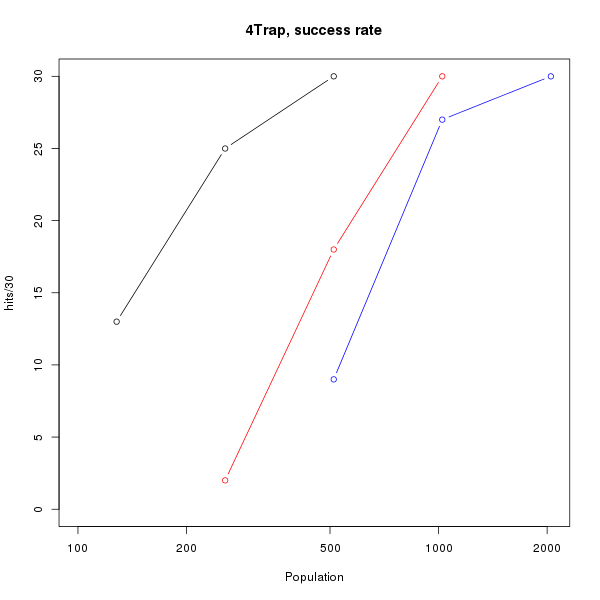
\includegraphics[scale=0.4]{base-hits-pop.png}
\caption{Number of successful runs out of 30; a run is considered
  successful if the target string (all ones) is found. The leftmost
  line corresponds to 30 blocks, the one in the middle to 40 and the
  last one to 50. }
\label{fig:pop}
\end{figure}
%
\begin{figure}[htb]
\centering
   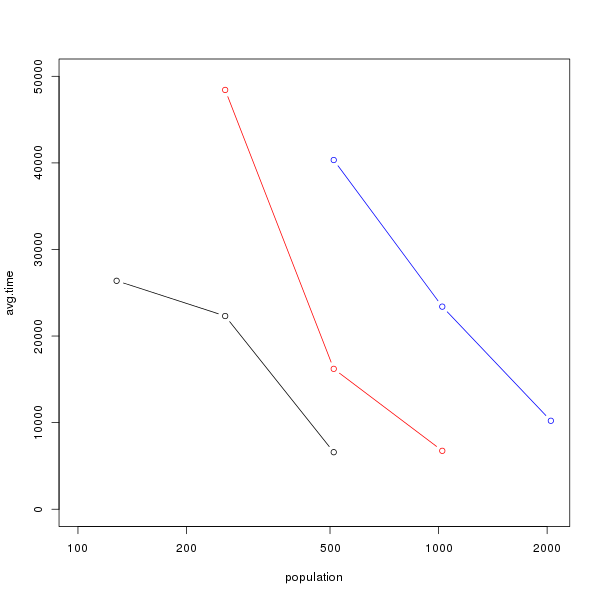
\includegraphics[scale=0.4]{base-time-pop.png}
\caption{Average time, in milliseconds, for successful runs. The leftmost
  line corresponds to 30 blocks, the one in the middle to 40 and the
  last one in the right to 50. }
\label{fig:time}
\end{figure}

The time needed to reach the solution follows a pattern that is
similar to the success rate, as shown in Figure \ref{fig:time}, which
plots the average time needed to find the solution in successful
runs. These graphs have two purposes: first, to show the time needed to
find the solution in Node, which is around 10 seconds for any of the
problems, slightly more for the problem with 50 traps. This time is
well in line with other script-based languages and show that
Javascript can be competitive, time wise, with other languages. As a
side comment, time decreases with population since the presence of a
higher initial diversity is key for a successful initial exploitation,
as opposed to an exploration regime that is needed to find the solution
with smaller sizes. We will also have to take into account this fact
when doing the parallel version of these algorithms, which we will
show in the next section.

It should be noted that the number of lines needed to implement this
problem is quite small and of the order of a few hundred of
lines. This fact, along with the performance obtained when solving
this problem, shows that JS and the library used in this paper
can be a contender in the arena of evolutionary computation
frameworks. 
% Antonio - quiz� har�a falta una comparativa con otras implementaciones o una REF para aseverar esto
However, the true worth of {\tt node.js} will be shown in the
next section by extending this basic algorithm for parallel execution.

\section{Testing distributed evolutionary architectures}
\label{sec:dist}

% Antonio - Interesar�a hacer una breve intro a los modelos distribuidos de EAs, o un par de citas. No todo el mundo en el GECCO los conocer�, creo yo. ;)

The easiest way of creating a distributed application using Node is
adding a RESTful interface to it using {\tt express.js}; in fact,
RESTful interfaces are quite efficient and have been tested already in
distributed EC experiments \cite{DBLP:journals/corr/abs-1105-4978},
finding that they add a small overhead to communications and, besides,
can be accessed from a variety of languages, from {\tt node.js} itself to
JQuery (a JavaScript library) in the browser. This gives us room for
growth, but for the time being we are interested only in showing that
a few lines of code can be used to convert a single-process
evolutionary algorithm into a distributed evolutionary one.

We will test two different regimes here:\begin{itemize}
\item {\em P2P}: in it, every {\em node} (which we will call
  process from now on, since they are implemented as such and to avoid
  confusion with {\tt node.js}, the JS interpreter) communicates with the
  rest.
\item {\em pool-based} communication of one client with other is only
  done through the server, with each program acting independently and
  knowing only about this server. 
\end{itemize}

These two implementations will be described in detail in the next two
sections, after which we will present and compare the result of the experiments
using them.

\subsection{P2P implementation}

Every program uses {\tt express.js} for implementing a response to GET
requests made by other processes. After a number of generations which
is configurable, a process makes a request to another process that is
selected randomly from the list of processes that are running the same
algorithm. Every process runs in its own port; these are assigned
sequentially starting by 3000; 4 processes, for instance, will use
ports 3000 to 3003. 

The queried peer returns the best chromosome in its pool. As pointed out 
in Section \ref{sec:node}, the chromosome is incorporated in a
later moment to the pool if the program does not finish before. The
new chromosome substitutes the last one in the pool, as it is usual. This
is the case too for the other regime. 

We call this implementation P2P, because every process is a client
(requesting individuals from other processes) and a server (serving
those requests). By default, all clients are stored at the same time
(except for negligible delays) using a shell script. 

Every process is run independently, which accounts for a high load of
the machine, approximately 1 per process. Even so, the operating
system is able to accommodate 16 processes without experimenting major
delays in the rest of the applications (such as music reproducer or
the browser) running on the server. 

\subsection{Pool-based implementation}

In this case, processes act only as clients, making GET and PUT
requests to a single server. This server runs in a public port (by
default, 5000) and handles all requests using {\tt express.js} integrated web
server. Since this server is asynchronous it is theoretically able to
serve a good amount of simultaneous requests. However, this number is
not infinite, as we will see later on. The client always PUTs the best
chromosome. 

The server provides a random chromosome when requested and when it
receives a PUT request it stores this in a hash, in such a way that if
the same chromosome is PUT twice it will be stored only once in the
server. This is mainly done for efficiency purposes, but also to increase
diversity. 

The client processes, after a fixed amount of generations, do a PUT
and then a GET. As explained in Section \ref{sec:node}, this does not
guarantee that they will be served in the same order so error-handling
provisions are in place in case the server has no chromosomes stored
(at the beginning of the simulation) or any other error (like a
flooding of the request buffer).

The server is started before the clients, which start all at the same
time (but see above). When all client processes have finished, the
server is killed so that no results are kept from one run to the next.

\subsection{Experiments and results}

First we will test if the approach is valid and if by dividing the
population in several processes we obtain any kind of improvement. The
machine is the same as above and except for some errors all
experiments have been repeated 30 times to achieve statistical
significance. In many cases, the {\em generational gap}, that is, the
number of generations before migration takes place, 
% Antonio - eso no se llama migration rate?
has been changed
to 10 or 20 if it was considered necessary; the point of the
experiment is, anyways, to see how the division of the population
influences the performance. 

\begin{figure}[htb]
\centering
   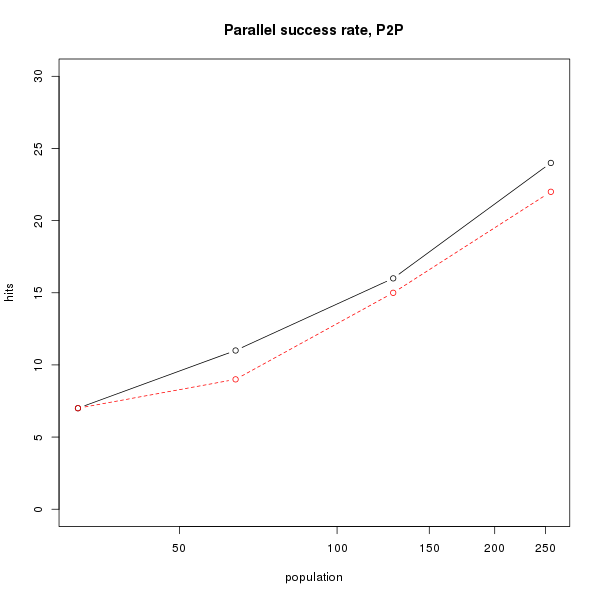
\includegraphics[scale=0.4]{parallel-hits-pop.png}
\caption{Number of successful runs out of 30. Black, solid line
  corresponds to migration after 20 generations, light-colored, dashed
corresponds to migration after 10 generations.}
\label{fig:p2p:hits}
\end{figure}
%
\begin{figure}[htb]
\centering
   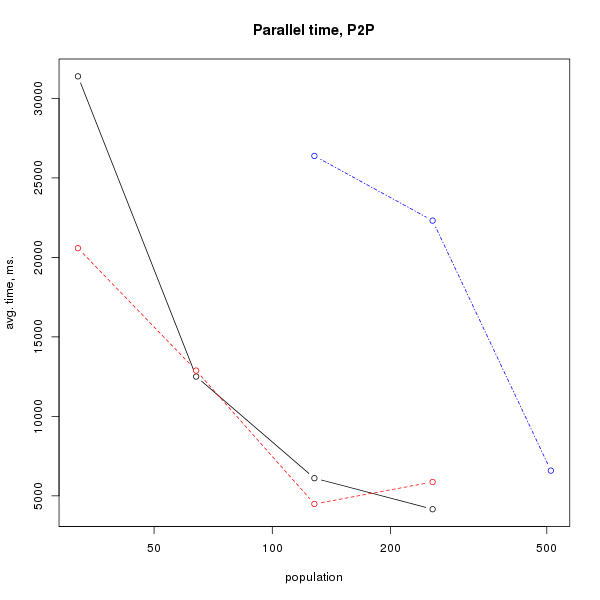
\includegraphics[scale=0.4]{parallel-time-pop.png}
\caption{Average time, in milliseconds, for successful runs. Black,
  solid line corresponds to $g$ (generation gap) = 10, light, dashed
  to $g=20$, and, for the sake of comparison, the baseline single-node
time is included. }
\label{fig:p2p:time}
\end{figure}

% Antonio - cambio 'node' por 'process', como indicaste antes para evitar confusiones con 'Node'
The success rate is shown in Figure \ref{fig:p2p:hits} for the 10 and
20 generation gap. The results are practically the same, and, in fact,
very similar to the success rate we would obtain with a single process; a
parallel division, in fact, does not seem to bring a improved success
rate even if the total population is the same as the one that obtained
100\% success in a single {\em deme}. The fact that a small variation
in the generation gap does not affect the time-to-success (when it is
achieved) is also reflected in Figure \ref{fig:p2p:time}, which also
shows the time in the single-process version that was presented in
Section \ref{sec:node}. It is interesting to see that time improves
5-fold for population = 256 (while the number of processes has only been
multiplied by two and success rate is roughly constant)  and roughly
in the same proportion for population = 128, with the number of
processes multiplied by 4. However, it is interesting to note that a
increase in the number of nodes from 256 to 128 does not decrease
running time and might even increase it. 

In fact, an additional experiment with 2 processes, $g=20$ and
population=512 confirms  what we have just seen above: success rate
remains 100\% but average time needed to find the solution decreases 3
times, to  1746 ms. from  6588.0 . This superlinear increase, which
has been found in many other experiments, might be due to the
asynchronous nature of Node, which might, in turn, increase
diversity, but in any case it proves that, in this P2P regime, adding
a single process might bring great improvements in terms of time, even in
a single machine. However, designing an experiment that proves this is
outside the scope of this paper and.

What we can conclude from this set of experiments is that a single
machine is able to support a good amount of processes running in
parallel, and that adding at least one process can increase speed
significantly without too much effort (a few lines of code) from the  programming point of view. 

However, this programming effort can be used in a different direction,
and that is what we have attempted with the pool architecture,
% Antonio - he puesto aqu� pool architecture en lugar de other architecture
 with
clients all working against a single server. In principle we wanted to
test the same architecture with the same generational gap, that is,
total population for all nodes equal to 512, with this population
divided among processes. However, since all the requests are done to a
single process its event queue saturates very fast which led us to
increase the generational gap with the number of processes; even so, it
brings errors which crash the clients in some cases.
% Antonio - si se han solucionado los problemas yo no lo comentar�a. ;)

\begin{figure}[htb]
\centering
   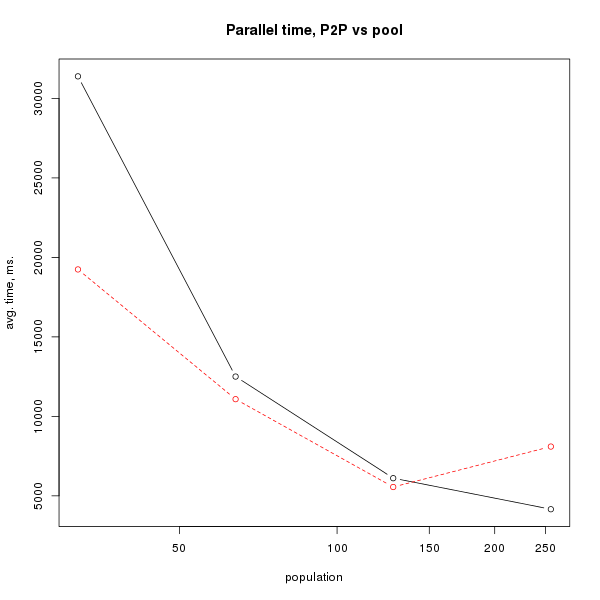
\includegraphics[scale=0.4]{par-pool-time-pop.png}
\caption{Average time, in milliseconds, for successful runs. Black,
  solid represents the previously mentioned P2P architecture, while
  the light, dashed line represents the pool-based, single-server
  architecture. }
\label{fig:p:time}
\end{figure}
%
\begin{figure}[htb]
\centering
   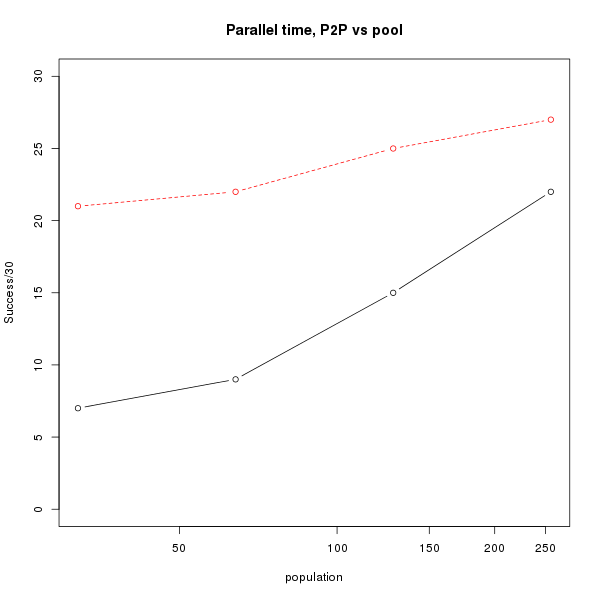
\includegraphics[scale=0.4]{par-pool-hits-pop.png}
\caption{Number of successful runs out of 30. Black, solid line
  corresponds to the P2P architecture, light-colored, dashed
corresponds to the single-server architecture (pool).}
\label{fig:p:hits}
\end{figure}
% Antonio - he puesto aqu� 'pool' porque las im�genes pueden salir lejos una de otra y as� son autocontenidas.


In general and from the point of view of the operating system load, no
great change is observed with the addition of one process ($n$ client
processes + server) to the pool; if there is any time difference, it
should not be attributed to increased OS load or, for that matter, for
the small changes in the application architecture done. Even if the
P2P applications do a single request (a GET) and this one performs two
(first a PUT and then a GET), it probably cancels out with the fact
that the P2P processes must also {\em respond} to requests from time
to time. In fact, what we observe in the comparison of both types of
architectures in Figure \ref{fig:p:time} is that there is a difference
for the smallest number of processes and the biggest number of
processes but they go in different directions, so it is difficult to
say if, in general, there is any difference (there is none for
$p=64,128$) and what is its origin. 

But a more dramatic change of scenario is shown in Figure
\ref{fig:p:hits}, which shows that the success rate increases
drastically, although decreasingly so with the increasing population;
this is only to be expected since, in fact, success rate increased
with the population in the P2P architecture. This makes, from the
algorithmic point of view, a better alternative of this pool-based
architecture. Since, time-wise, there is no big difference, we have to
conclude that, in general and despite server-overload errors, using a
pool-based architecture for asynchronous parallel evolutionary
algorithms is a better option than either a single-population
architecture or a peer-based architecture. 

This conclusion is reached on top of the fact that JavaScript, its
implementation in {\tt node.js}, and the simple library we are presenting in
this paper, are valid platforms for performing distributed computation
experiments, since they allow to create rapid prototypes to
concentrate on system architecture and the solution of problems via
evolutionary algorithms. In an unconstrained environment, Javascript will probably be slower than Java or C++, although its speed is on par (and may beat) other scripting languages. However, in an environment such as a multi-tier architecture that includes rich internet applications (with an UI written in JavaScript in the browser) or even mobile applications (which can easily be done in JavaScript via the PhoneGap framework or simply HTML5 in any browser) JavaScript can offer an excellent performance and even algorithmic advantages in parallel evolutionary algorithms, as we have proved in this paper. 

% Antonio - Creo hay que darle m�s bombo a esto porque el objetivo del trabajo parec�a ser que ofrec�a una alternativa MEJOR a lo que ya hay, es decir, mejor que las implementaciones de EAs en C y Java por ejemplo, pero eso no se comenta, s�lo se dice que JavaScript ofrece una implementaci�n V�LIDA... queda un poco flojo en ese sentido. :-(


\section{Conclusions}

In this paper we set to prove the worth of a {\tt node.js}-based distributed
evolutionary algorithm. {\tt node.js} is a emerging platform which is
receiving a lot of interest in the open source and enterprise arena,
but not so much in the scientific community so our intention was to
introduce it to the evolutionary computation (EC) community by proving its
value as a platform for EC experiments. A basic EC library has been
created and released, so it is available to the researches. The
library can be expanded and, being open source, can be adapted and
suited to the needs of any particular user; due to the expansion of
the JavaScript and {\tt node.js} community, it should be increasingly easy
to find people interested and skilled enough to work in evolutionary
algorithms using JavaScript and {\tt node.js}, and, from the other end, it could get
the {\tt node.js} community interested in our area, which might prove the
source of interesting problems that can be dealt with from the point
of view of metaheuristics.

The main challenge of this paper was to create evolutionary algorithms
program that took advantage of the asynchronous nature of {\tt node.js} and
the easiness with which asynchronous communication is done using
it. To that end, two implementations of a parallel system (that can be
easily distributed by changing the configuration files of the clients
to reflect the URLs used), one in which evolutionary islands form a
{\em star} topology 
% Antonio - REF?
and are aware and communicate with all other
processes, and another in which each client must be aware only of the
server it uses to deposit and pick up individuals that are deposited
by other clients. These two alternatives offer different advantages
from the raw and algorithmic performance point of view: while the P2P
setup is able to achieve great improvements by reaching solution in a
portion of the time, the server-based setup not only offers
improvements of the same order, but also is able to improve the
success rate over the P2P and single-server architecture. This despite
the disadvantage of the server not being able to process all requests
in some occasions.

Why this happens is, however, a different matter. The P2P system
always deposits the best individual in the current generation and
retrieves also the best from its peer. This might not be the best
alternative, as shown in papers such as
\cite{multikulti:cec09}. However, the peer it takes the chromosome
from {\em is} random, so that might not be the problem. It would be
interesting, however, to use other strategies to retrieve individuals
from other processes to check what is exactly the reason for this lack
of performance. On the other hand, the pool-based system retrieves a
random individual from the pool, but this individual has been, in some
past moment, the best since they only deposit the best, so the
probably increase in diversity afforded by using a random individual
from the server might not be the reason; in fact, this was chosen
since retrieving the best would probably get the same individual the
client had just deposited and checking for that might lead to
increasing complexity that we pointedly tried to avoid. 

In any case, it is quite clear that the use of this platform and the
degrees of liberty in its design open a whole world of possibilities
to test, including these \begin{itemize}
\item Uniform vs. heterogeneous settings in nodes. We have been using a
  single population size, generation gap and tournament size, in
  general. Using dissimilar and even random values might increase
  diversity and thus increase the success rate.
\item Heterogeneous systems vs. homogeneous systems: using the same
  parameters in different systems will, once again, increase diversity
  and will allow anyways the use of many more resources that are
  available under a single motherboard. Using free PaaS (Platform as a Service) or the free
  tier of IaaS (Infrastructure as a Service) products such as Amazon EC2 or Azure will allow to work
  with bigger problems, be it in a P2P or pool-based fashion
\item The P2P and pool-based options are not mutually exclusive, since
  in fact the program used in the P2P setup can be used as a server by
  adding to it the capability to respond to PUT petitions. Working
  with different servers and distributing clients might offer a way
  out of the server overload problem but, at the same time, opens many
  more possibilities.
\end{itemize}

We should emphasize too that this research has been carried out in an
open science fashion by publishing, as soon as they are produced, all
results on a public server whose address is withheld at this point in
the evaluation on the paper. We have made sure that these results are
fully reproducible by not only releasing the source code, but also
all configuration files (in JSON) and data obtained during the
experiments, as well as a configuration script in Ansible for the
setup of a virtual or real machine.


%ACKNOWLEDGMENTS are optionalndn
\section{Acknowledgments}

Withheld for anonymous review \\
but\\
should have these many lines.

%Este trabajo se est� desarrollando gracias a la financiaci�n de  los
%proyectos CANUBE (CEI2013-P-14) y ANYSELF (TIN2011-28627-C04-02). 

%
% The following two commands are all you need in the
% initial runs of your .tex file to
% produce the bibliography for the citations in your paper.
\bibliographystyle{abbrv}
\bibliography{geneura,javascript,ror-js}  % sigproc.bib is the name of the Bibliography in this case

\end{document}
